


\documentclass{beamer}

\mode<presentation>{
%\usetheme{default}
%\usetheme{AnnArbor}
%\usetheme{Antibes}
%\usetheme{Bergen}
%\usetheme{Berkeley}
%\usetheme{Berlin}
%\usetheme{Boadilla}
%\usetheme{CambridgeUS}
%\usetheme{Copenhagen}
%\usetheme{Darmstadt}
%\usetheme{Dresden}
%\usetheme{Frankfurt}
%\usetheme{Goettingen}
%\usetheme{Hannover}
%\usetheme{Ilmenau}
%\usetheme{JuanLesPins}
%\usetheme{Luebeck}
%\usetheme{Madrid}
%\usetheme{Malmoe}
%\usetheme{Marburg}
%\usetheme{Montpellier}
%\usetheme{PaloAlto}
%\usetheme{Pittsburgh}
%\usetheme{Rochester}
%\usetheme{Singapore}
%\usetheme{Szeged}
\usetheme{Warsaw}

%\usecolortheme{albatross}
%\usecolortheme{beaver}
%\usecolortheme{beetle}
%\usecolortheme{crane}
%\usecolortheme{dolphin}
%\usecolortheme{dove}
%\usecolortheme{fly}
\usecolortheme{lily}
%\usecolortheme{orchid}
%\usecolortheme{rose}
%\usecolortheme{seagull}
%\usecolortheme{seahorse}
%\usecolortheme{whale}
%\usecolortheme{wolverine}
}

\usepackage[brazil,american]{babel}
\usepackage[T1]{fontenc}
\usepackage{indentfirst}
\usepackage{natbib}
\usepackage{xcolor,graphicx,url}
\usepackage{subcaption}
\usepackage[utf8]{inputenc}

\graphicspath{ {imagens/} }



%-----SLIDE DO TITULO-----%

\title[Seminario TG1]{Detecção e monitoramento de vagas de estacionamento através de visão computacional}
\author{Vitor de Alencastro Lacerda - 11/0067142}
\institute[UnB]{
    Universidade de Brasília
    \medskip
}
\date{\today}

%--------------------------%

\begin{document}


\begin{frame}
\titlepage
\end{frame}

\begin{frame}
\frametitle{Roteiro} % Table of contents slide, comment this block out to remove it
\tableofcontents % Throughout your presentation, if you choose to use \section{} and \subsection{} commands, these will automatically be printed on this slide as an overview of your presentation
\end{frame}


\AtBeginSection[]
{
\begin{frame}{Table of Contents}
\tableofcontents[currentsection]
\end{frame}
}

%-----APRESENTACAO MESMO------%


\section{Revisão Teórica}
\begin{frame}
\frametitle{Processamento de Imagens}
\begin{itemize}
  \item Área da computação derivada do processamento de sinais.
  \item Aprimoramento de imagens para interpretação humana
  \item Algoritmos para análise automática de informações em uma imagem.(Visão computacional)
\end{itemize}

\end{frame}
\begin{frame}
\frametitle{Subtração de imagens}
\begin{itemize}
  \item Uma imagem é representada por um conjunto de pixels em um espaço cartesiano
  \item Consiste em extrair uma imagem  de diferença entre duas imagens através da subtração de valores nas mesmas coordenadas
  \item Usada para extrair diferenças entre quadros
\end{itemize}

\begin{equation}\label{diferenca}
  D(x,y) = A(x,y) - B(x,y)
\end{equation}

\end{frame}
\begin{frame}
\frametitle{Geração de fundo}
\begin{itemize}
  \item Processo que envolve separação entre o foreground e o background de um video.
  \item Background - Objetos estáticos
  \item Foreground - Objetos em movimento
\end{itemize}

\end{frame}
\begin{frame}
\frametitle{Histogramas}
\begin{block}{Histograma}
Uma representação da distribuição dos valores dos pixels de uma imagem. Normalmente representado com um gráfico de barras.
\end{block}

\begin{figure}
  \centering
  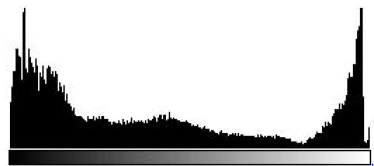
\includegraphics[width=.4\textwidth]{Histograma2}
\end{figure}

\end{frame}



\section{Problema e motivação}

\begin{frame}
\frametitle{Problema}

\begin{block}{Problema}
    Há uma falta no mercado de sistemas que sejam capazes de monitorar e gerenciar vagas em estacionamentos ao ar livre.
\end{block}
\end{frame}

\begin{frame}
 \frametitle{Hipoteses}
 \begin{itemize}
   \item  As soluções para estacionamento fechados não são utilizadas nos estacionamentos abertos porque são caras, difíceis de instalar e de difícil escalabilidade.
   \item  Utilizar algoritmos de visão computacional é uma solução barata, eficiente e eficaz para realizar esse monitoramento.
   \item  É possível utilizar técnicas de geração de fundo para separar veículos em movimento
   \item  É possível usar essa informação e diferenças entre fundos para determinar estados de vagas de estacionamento.
 \end{itemize}
\end{frame}

\begin{frame}
\frametitle{Motivacao}
Motivações para o trabalho:
\begin{itemize}
  \item Financeira: Rondar estacionamentos em busca de vagas gasta tempo e dinheiro.
  \item Comercial: Sistema atrai clientes e automatiza gerência de estacionamentos rotativos.
  \item Mercado: Soluções que existem atualmentes não são adequadas para estacionamentos abertos.
\end{itemize}

\end{frame}


\section{Objetivos}
\begin{frame}
\frametitle{Objetivos}
\begin{block}{Objetivo Geral}
Desenvolver um sistema capaz de analisar imagens de uma câmera de vídeo para identificar vagas vazias e ocupadas em um estacionamento descoberto e informar aos usuários e donos do estacionamento.
\end{block}

\end{frame}
\begin{frame}
\frametitle{Objetivos}
Objetivos específicos:
\begin{itemize}
  \item Detectar automaticamente as vagas do estacionamento.
  \item Determinar informações adicionais sobre o estacionamento
  \item Fornecer funções para automatizar a gerência de estacionamentos rotativos.
\end{itemize}

\end{frame}
\begin{frame}
\frametitle{Objetivos}
\begin{block}{Resultado Esperado}
Um sistema barato e eficiente que seja capaz de facilitar a vida de usuários de estacionamentos e automatizar a gerência em estacionamentos rotativos.
\end{block}
\end{frame}




\section{Metodologia}

\begin{frame}
\frametitle{Metodologia}
    \begin{block}{Aquisição das imagens}
    Os primeiros testes do trabalho serão feitos sobre imagens criadas artificialmente. Alguns em imagens estáticas e outros em vídeos criados através de manipulação de imagens. Futuramente, vídeos reais serão analisados.
    \end{block}
\end{frame}

\begin{frame}
\frametitle{Metodologia}
    Passos de funcionamento do programa:
    \begin{itemize}
        \item Extração do fundo
        \item Subtração de fundos distintos
        \item Identificação de objetos
    \end{itemize}
\end{frame}

\begin{frame}
\frametitle{Metodologia}
O fundo deve ser gerado de forma dinânica por causa das seguintes dificuldades:
\begin{itemize}
  \item Mudança na iluminação durante o dia
  \item Ruído da imagem
  \item Clima
  \item Objetos novos que podem se integrar ao fundo
\end{itemize}
\end{frame}

\begin{frame}
\frametitle{Metodologia}
    Começa de um fundo inicial.
    Gera o fundo a cada quadro de vídeo segundo a equação:
    \begin{equation}\label{geracaoFundoEquacao}
       Bgi = \left\{
        \begin{array}{l l}
        Ba_{i} & \text{,Fgi=255} \\
        \frac{Bai}{2} + \frac{Qi}{2} & \text{,Fgi=0}\\
         \end{array} \right.
     \end{equation}
\end{frame}

\begin{frame}
\frametitle{Metodologia}
   \begin{figure}
      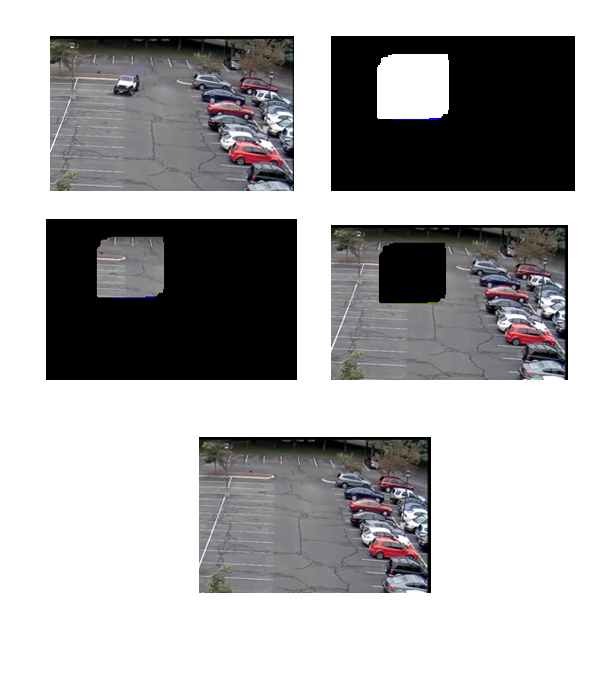
\includegraphics[width=.6\textwidth]{FiguraFundo}
    \end{figure}
\end{frame}

\begin{frame}
\frametitle{Metodologia}
   A cada intervalo de tempo $t$, o fundo atual é subtraído do fundo de $t$ segundos atrás.

   As imagens de diferença são tratadas para excluir diferenças insiginificantes.

   Diferenças podem significar duas coisas:
   \begin{itemize}
        \item Um novo objeto se integrou ao fundo ou;
        \item Um objeto estático saiu da imagem.
    \end{itemize}
\end{frame}

\begin{frame}
\frametitle{Metodologia}
   O próximo passo é comparar a região da diferença com as posições conhecidas de vagas e determinar se a vaga foi ocupada ou desocupada.

   Se o estado anterior é conhecido e apenas carros pudessem se integrar ao fundo, isso seria trivial, mas esse não é o caso.

    Também é preciso identificar que o objeto representado na diferença é realmente um carro.
\end{frame}

\begin{frame}
\frametitle{Metodologia}
   Métodos sendo explorados:
   \begin{itemize}
     \item  Rastreamento
     \item  Comparação de histogramas
     \item  Classificação
   \end{itemize}
\end{frame}

\begin{frame}
\frametitle{Plano de implementação}
   A implementação vai seguir os seguintes passos:
   \begin{itemize}
     \item  Determinar ocupação de vagas em imagens estáticas a partir de um estado inicial conhecido e subtração de imagens.
     \item  Determinar o estado das vagas a partir apenas de uma imagem.
     \item  Usar o segundo passo para conferir os estados obtidos no primeiro passo.
     \item  Implementar os métodos desenvolvidos nos passos anteriores em vídeos 'artificiais'.
     \item  Validar o funcionamento do programa em vídeos reais.
   \end{itemize}
\end{frame}

\section{Cronograma}
\begin{frame}
\frametitle{Cronograma 2015}
%
\begin{tabular}{|l|c|c|c|c|c|c|c|}
\hline
Atividade & Jan & Fev & Mar & Abr & Maio & Jun & Jul \\
\hline
Pesquisa & X & X & & & & &  \\
\hline
Imagens &  & X & X &  &  &  &   \\
\hline
Implementação&  & X & X & X &  &  &   \\
\hline
Validação &   &   &  & X & X &  &   \\
\hline
Análise &   &   &  & X & X & X &   \\
\hline
Escrita  &   &   &  &  & X & X &   \\
\hline
Defesa  &   &   &  &  &  &  & X  \\
\hline
\end{tabular}
%



\end{frame}




\section{Conclusao}
\begin{frame}
\frametitle{Conclusao}
\huge
Perguntas?

\end{frame}


\begin{frame}[allowframebreaks]
\frametitle{Referencias}
\bibliographystyle{plain}
\bibliography{bibliografia}

\end{frame}




\begin{frame}
\frametitle{Conclusao}
\huge
\cite{bong2008integrated} \cite{chen2012dynamic} \cite{de2006introduccao} \cite{delibaltov2013parking}\cite{gonzalez2009digital}
\cite{graciano2007rastreamento} \cite{hai2009self} \cite{IBGE2000introducao} \cite{idris09} \cite{marques1999processamento}
\cite{true2007vacant} \cite{vkl1989jain}
\end{frame}


%------------------------------%


\end{document} 